\chapter{Dark matter and dark energy}

\section{Introduction}

In lecture 6 we started our study of the energy content of the universe, and we showed how the different contributions to the total energy density evolve in time in the context of the Big Bang model. In particular, we have seen that these contributions can be divided into three classes: radiation, matter, and dark energy. The matter itself can be further divided into baryonic (ordinary) matter and dark matter. At the present time ($t=t_0$), the experimentally measured density parameters are given by\footnote{Here we omit the experimental errors in these quantities, which are presently fairly large. So do not be surprised if you see slightly different numbers in different books.}
\begin{equation} \label{eq:dens_param_today}
\begin{split}
\Omega_{b}(t_0)&\approx 0.04,\\
\Omega_{DM}(t_0)&\approx 0.22,\\
\Omega_{\Lambda}(t_0)&\approx 0.74,
\end{split}
\end{equation}
in addition to the photon and neutrino density parameters, which give a very small contribution ($\Omega_{\gamma},\Omega_{\nu}\sim10^{-5}$) today. Given that, experimentally (and as predicted by theory of inflation), the total density parameter is very close to unity, $\Omega(t_0)\approx 1$, we can translate the numbers in eq.\ (\ref{eq:dens_param_today}) to the percentages corresponding to the different energy contributions in the universe. These are shown in fig.\ \ref{fig:lec10_1}.
\begin{figure}[ht]
\begin{center}
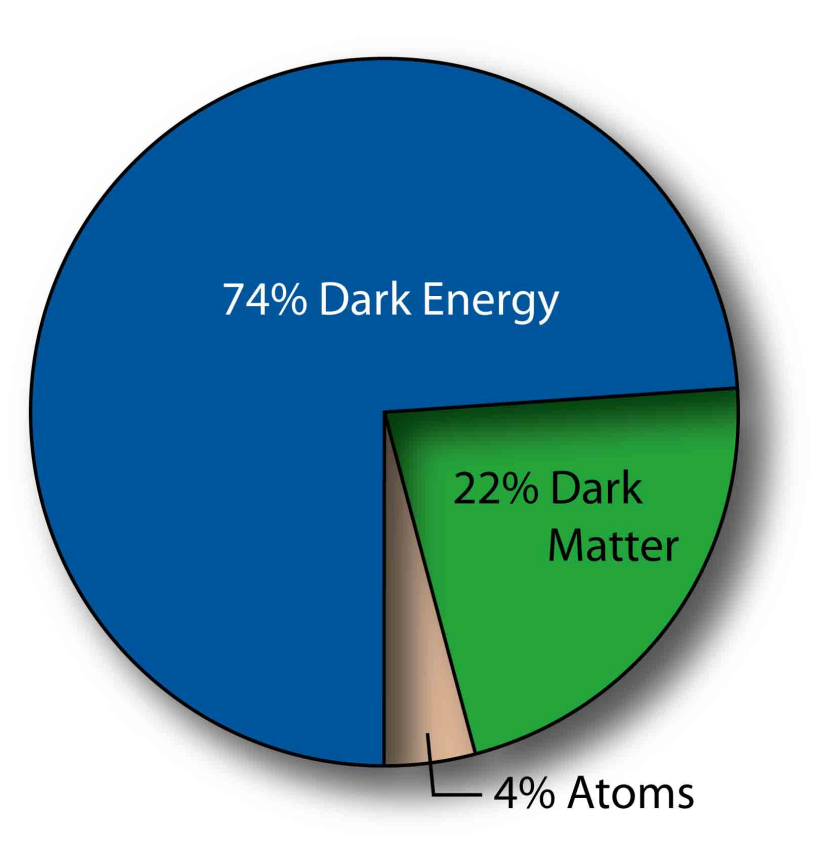
\includegraphics[scale=2]{Draw/lec10_1.png}
\end{center}
\caption{Energy content of the present universe (Source: \url{http://xenon.physics.rice.edu})}
\label{fig:lec10_1}
\end{figure}

The important and striking conclusion that one can draw from this chart is very clear: $96\%$ of the universe is in the form of dark matter and dark energy, which are two forms of energy whose exact nature is unknown. The most widely accepted explanation among physicists (we will see that there are others though) is that dark matter is really matter, meaning that it is some kind of particle. The problem, however, is that none of the particles found in the Standard Model of particle physics can possibly be the dark matter. Far more misterious is dark energy, whose behavior makes clear that it cannot be a particle or any other kind of energy known to physicists.

The goal of this lecture is to provide an overview of the experimental evidence for the existence of dark matter and dark energy, and to introduce some (but certainly not all) of the theories that could potentially explain what they are.

\section{Dark matter}

\subsection{Observational evidence}

We begin by studying the astronomical evidence that supports the existence of dark matter. This evidence shows up in a number of different contexts, thus providing a very complete picture of the role of dark matter in cosmology and astrophysics.

\subsubsection{Cosmological evidence}

We have seen in the previous lecture that there is a lot to learn from the CMB power spectrum. More specifically, the locations and shapes of the acoustic peaks (see fig.\ \ref{simpow}) depend on quantities that are directly determined by the cosmological density parameters. For instance, one can show that the location of the first acoustic peak is a good indicator of the spatial curvature of the universe. Specifically, in a negatively curved universe ($k=-1$) the first acoustic peak should correspond to a multipole moment $l\gtrsim200$, whereas in a positively curved universe ($k=+1$) the peak should occur at $l\lesssim200$. The fact that we observe this first peak precisely at $l\simeq200$ implies that the universe must be spatially flat ($k=0$) or very nearly so ($k/R^2\approx0$, where $R$ is the radius of curvature). In lecture 6 we showed that the Friedmann equation implies the relation
\begin{equation}
\frac{k}{R^2}=\frac{H_0^2}{c^2}\left(\Omega(t_0)-1\right).
\end{equation}
If the left-hand side of this relation is close to zero, as suggested by the CMB power spectrum, then so must be the right-hand side. From this we can conclude that
\begin{equation}
\Omega(t_0)\approx 1.
\end{equation}

A second piece of information that allows us to constrain the density parameters comes from the observations of type Ia supernovae, which provide an independent measurement of the density parameter of dark energy, $\Omega_{\Lambda}$ (we will come back to this in the next section). Type Ia supernovae are different from the more usual supernovae that result from the gravitational collapse of very massive stars. Rather, they result from the collapse of white dwarfs that reach a critical mass by accreting gas from a companion star (fig.\ \ref{fig:lec10_3}).
\begin{figure}[ht]
\begin{center}
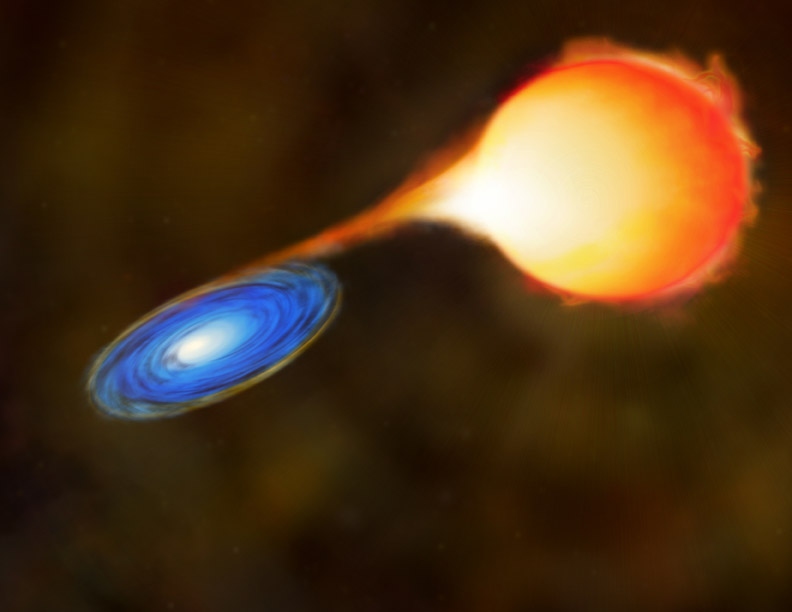
\includegraphics[scale=0.3]{Draw/lec10_3.png}
\end{center}
\caption{Artist conception of a supernova Ia (Image credit: NASA/CXC/M.\ Weiss)}
\label{fig:lec10_3}
\end{figure}

Type Ia supernovae are useful in cosmology because they are good {\it standard candles}, which are astronomical objects whose intrinsic luminosity can be estimated with good accuracy. Standard candles can therefore be used to measure distances: if we compare the apparent brightness of a supernova Ia (which depends on the location of the observer) with its luminosity (which is an intrinsic quantity), we can obtain a measurement of its distance.
\begin{figure}[ht]
\begin{center}
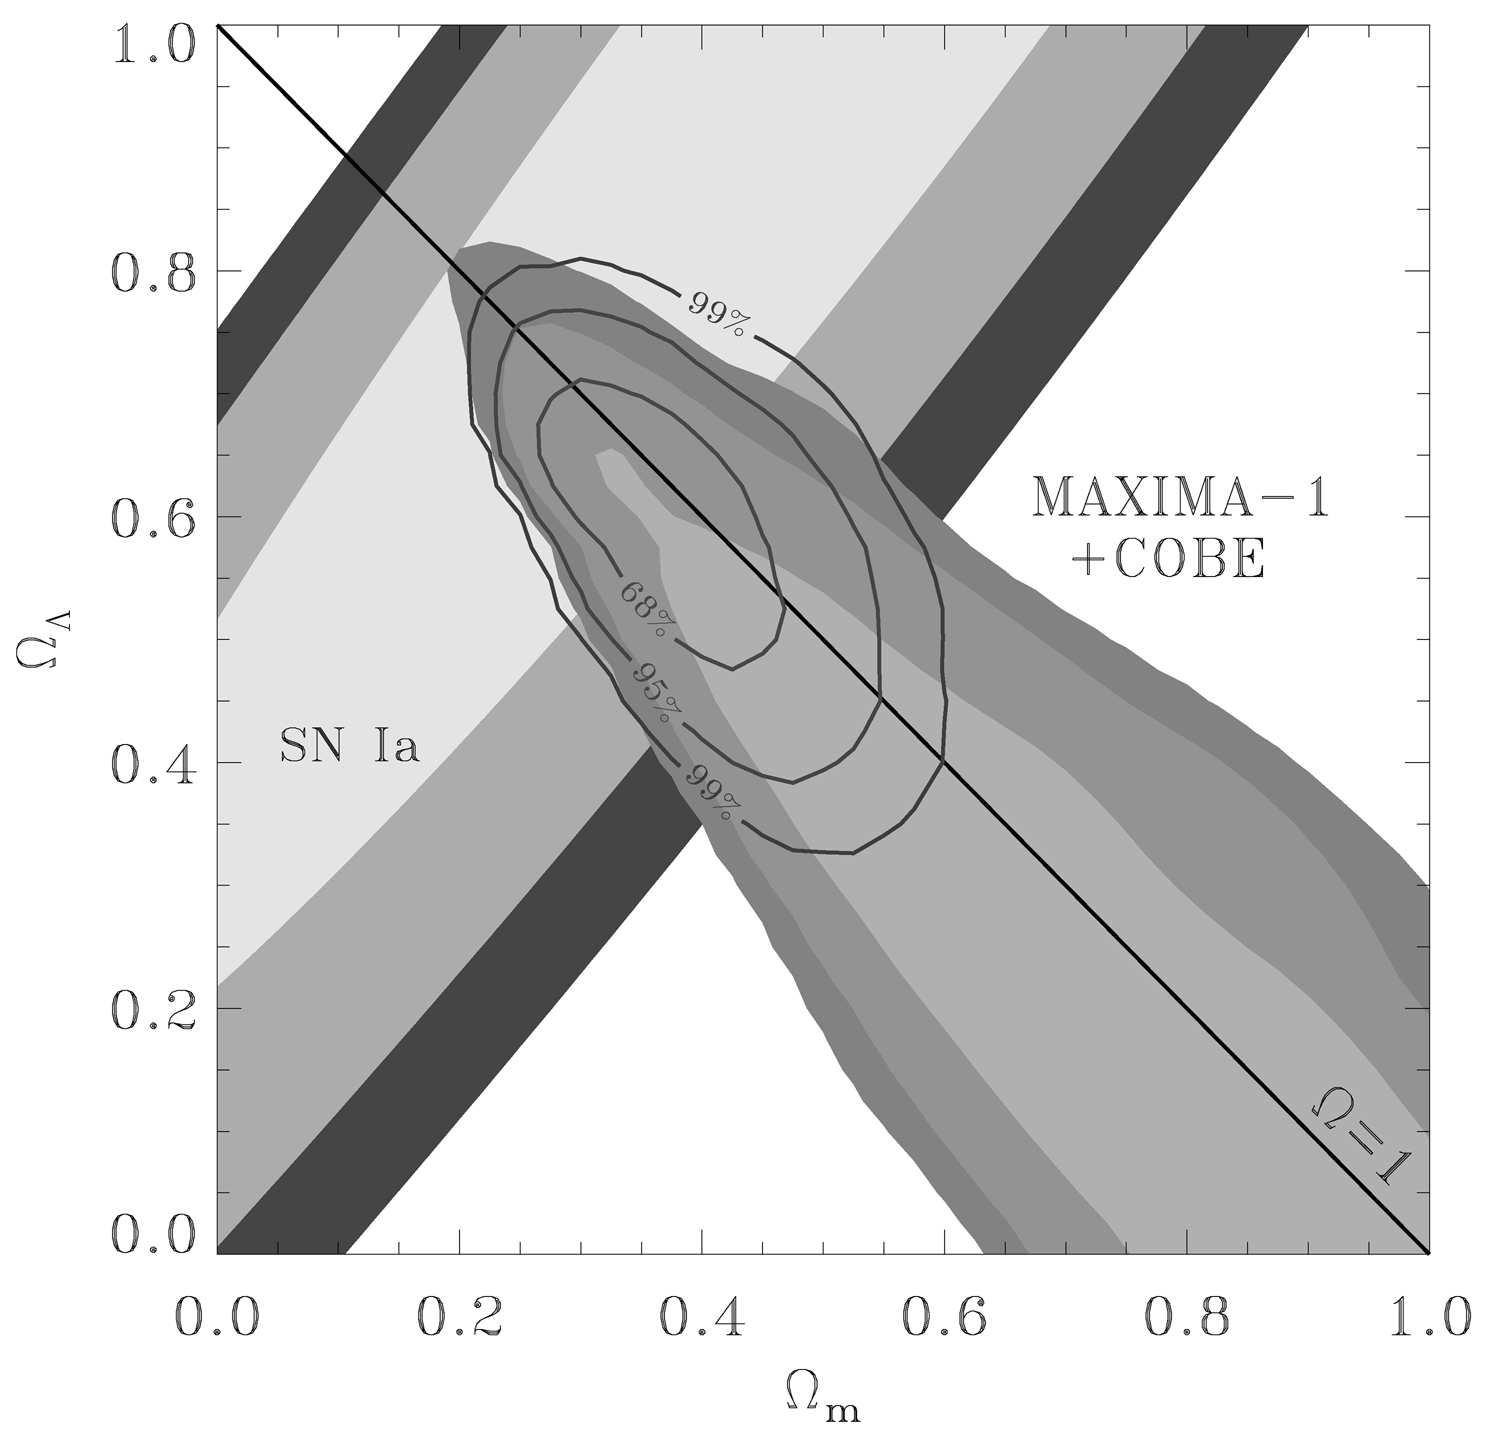
\includegraphics[scale=0.25]{Draw/lec10_2.png}
\end{center}
\caption{Energy content of the present universe (Image credit: Stompor et al., ApJ, 561, 2001)}
\label{fig:lec10_2}
\end{figure}

After combining the data from observations of the CMB and type Ia supernovae (see fig.\ \ref{fig:lec10_2}), cosmologists have been able to measure the present values of the matter density parameter, $\Omega_m(t_0)$, and the dark energy density parameter, $\Omega_{\Lambda}(t_0)$. The currently accepted values are approximately given by
\begin{equation}
\begin{split}
\Omega_m(t_0)&\approx 0.26,\\
\Omega_{\Lambda}(t_0)&\approx 0.74.
\end{split}
\end{equation}

Finally, a third piece of information comes from the independent measurement of the amount of baryonic matter in the present universe. Without going into the details, we can identify three methods by which physicists have been able to constrain the value of $\Omega_b(t_0)$, the baryonic density parameter today.
\begin{itemize}
\item The first method is conceptually very simple. We know that most of the baryonic matter is, in the present universe, contained in stars and in the intergalactic gas, so by measuring their average densities (over cosmological scales) one can estimate $\Omega_b(t_0)$. The average density of matter in stars can be estimated from the knowledge of the average number of galaxies per unit volume, and the average number of stars in a galaxy, which in turn can be measured by observing the luminosity of galaxies in optical wavelengths (which is mostly due to the stars). On the other hand, the mass density of the intergalactic gas can be measured from the observation of galaxy clusters in x-rays.
\item The second method is more indirect, and consists of comparing the presently observed abundance of heavy elements with the predictions of nucleosynthesis. The abundance of heavy elements can be estimated by observing the amounts of deuterium, helium, and lithium in primordial gas clouds. This abundance can be related to the efficiency of nucleosynthesis, which in turn can be related to the baryonic density.
\item Finally, a third method comes again from the first acoustic peak of the CMB power spectrum. It turns out that not only is the {\it location} of this peak useful for measuring cosmological parameters, but also its {\it amplitude} can be used to estimate, among other things, the baryonic density parameter $\Omega_b(t_0)$.
\end{itemize}

All these methods are consistent with a value of the density parameter of baryonic matter that is approximately given by
\begin{equation}
\Omega_b(t_0)\approx 0.04.
\end{equation}
This means that, of the total matter density parameter of $0.26$, only $0.04$ (or a $15\%$) corresponds to the ordinary baryonic matter. It follows that the remaining part ($85\%$ of the total matter) must be in the form of dark matter:
\begin{equation}
\Omega_{DM}(t_0)\approx 0.22.
\end{equation}

\subsubsection{Evidence from the large-scale structure}

Observations of the large-scale structure of the present universe provide a second piece of evidence for the existence of dark matter. Indeed, these observations show that dark matter was a crucial ingredient in the process of structure formation. We have seen in lecture 8 that, assuming a homogeneous background universe, inhomogeneities in the baryonic matter should grow proportional to $t^{2/3}$ after recombination. However, such a growth rate would be too slow to explain the matter structures that we observe in the present universe. The solution to this problem is that, in fact, the background in which the baryonic inhomogeneities evolve is actually not homogeneous, but already contains structures made of dark matter. This is because dark matter inhomogeneities begin to grow as soon as the universe becomes matter dominated, and so by the end of recombination dark matter structures already exist, and they enhance the growth rate of the baryonic inhomogeneities by providing an additional gravitational 
attraction. This process is shown schematically in fig.\ \ref{fig:lec8_5}.

\subsubsection{Evidence of dark matter in galaxies}

Consider a star near the outer edge of a spiral galaxy, moving with speed $v$ at a distance $R$ from the center of the galaxy. We would like to find how $v$ depends on $R$. For this we can assume that the star moves in a circular orbit, which is an accurate assumption for most stars in spiral galaxies. Then we can equate the centripetal force
\begin{equation}
F_c=m\frac{v^2}{R},
\end{equation}
with the gravitational force
\begin{equation}
F_g=\frac{GmM(R)}{R^2}.
\end{equation}
In these equations $m$ is the mass of the star, and $M(R)$ is the mass of the galaxy contained within the radius $R$. Notice that we can safely apply Newtonian mechanics here, since the speeds of stars are nonrelativistic. A further simplification comes from the fact that, for spiral galaxies, most of the stars are located within a radius $R_s$, known as the {\it scale radius}. It has a value of $R_s\sim 3-7$ kpc for most galaxies. This fact implies that for $R>R_s$ we can approximate $M(R)\approx M$, with $M$ the total mass of the galaxy. Then, equating $F_c$ and $F_g$, and assuming that the star is moving at a radius $R>R_s$, we obtain
\begin{equation}
\begin{split}
m\frac{v^2}{R}&= \frac{GmM(R)}{R^2}\\
v&= \sqrt{\frac{GM}{R}}
\end{split}
\end{equation}
\begin{equation} \label{eq:keplerian_rot}
\Rightarrow~~~~ v\propto \frac{1}{\sqrt{R}}.
\end{equation}
This dependence of the rotational speed $v$ on the radius $R$ is called {\it Keplerian rotation}. However, it turns out that this result does not agree at all with observations. By measuring the rotational speeds of stars in several spiral galaxies astronomers have found that, in fact, $v\propto\mathrm{const.}$ at radii $R>R_s$ (fig.\ \ref{fig:lec10_4}).
\begin{figure}[ht]
\begin{center}
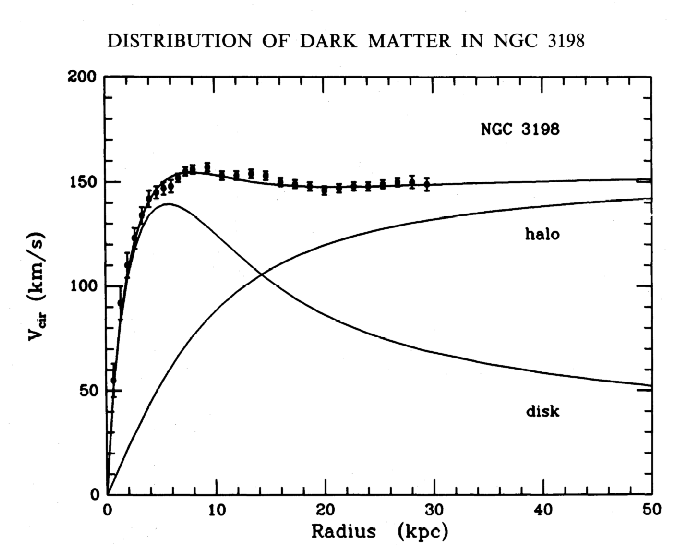
\includegraphics[scale=0.55]{Draw/lec10_4.png}
\end{center}
\caption{Rotation curve of galaxy NGC 3198 (Image credit: Van Albada et al., ApJ, 295, 1985)}
\label{fig:lec10_4}
\end{figure}

It is clear that one of the assumptions we made in our derivation of eq.\ (\ref{eq:keplerian_rot}) must be wrong. The most widely accepted explanation is the following. Although it is true that most of the stars are contained within a radius $R_s$ in spiral galaxies, it is not true that most of the {\it mass} is enclosed by this radius. However, we know that nearly all the {\it visible mass} is in fact given by the stars (the remaining fraction given by the interstellar gas),\footnote{By ``visible mass'' we mean the mass that interacts with electromagnetic radiation, but not necessarily in the visible spectrum.} so it must be true that there exists some {\it invisible mass} that extends beyond the scale radius of the galaxy. This invisible mass corresponds, of course, to the dark matter, and detailed studies have allowed astronomers to conclude that all galaxies are surrounded by a {\it dark matter halo}. This halo usually has a roughly spherical shape, and extends to distances several times larger than the 
size of the visible galaxy that it contains (fig.\ \ref{fig:lec10_5}).
\begin{figure}[ht]
\begin{center}
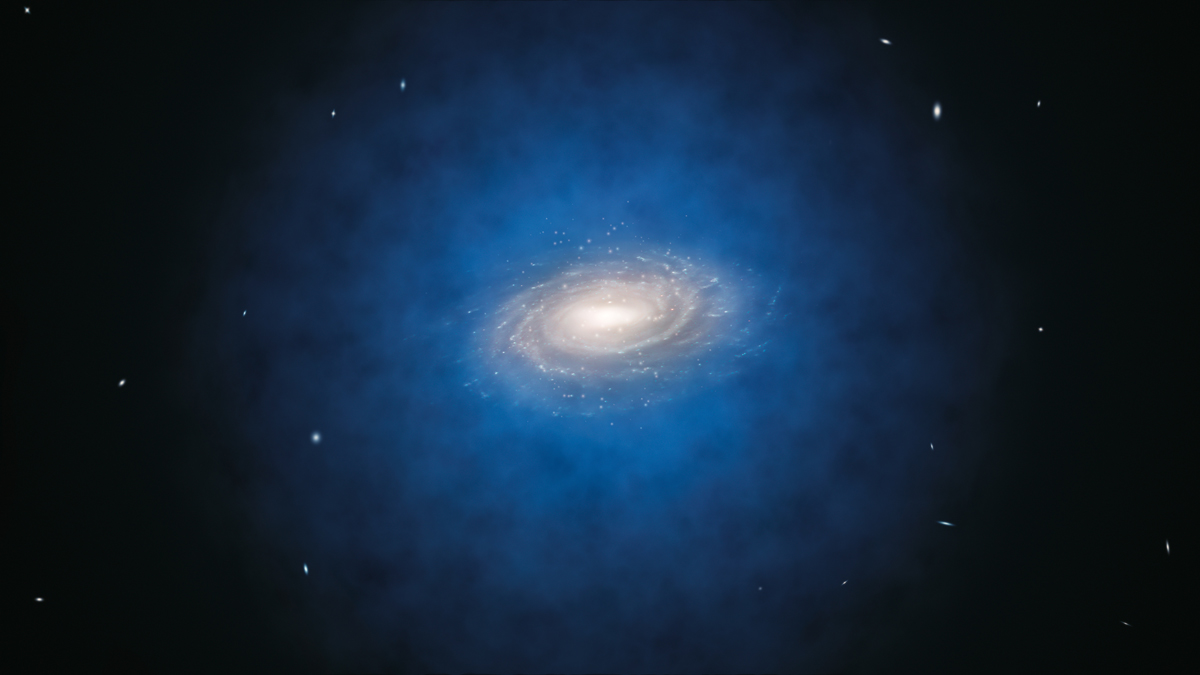
\includegraphics[scale=0.4]{Draw/lec10_5.png}
\end{center}
\caption{Artist impression of a dark matter halo (Image credit: ESO/L.\ Cal\c{c}ada)}
\label{fig:lec10_5}
\end{figure}

\subsubsection{Evidence of dark matter in galaxy clusters}

Further evidence for the existence of dark matter comes from studying the masses of galaxy clusters. For nearby clusters, it is possible to separately measure the visible mass, $M_{\mathrm{visible}}$, and the total mass, $M_{\mathrm{total}}$. The visible mass is given by the mass of the galaxies in the cluster plus the mass contained in the intergalactic gas, both of which can be directly measured. The mass of the galaxies can be estimated from observations of the luminosity of a cluster in optical wavelenghts, while the mass of the intergalactic gas can be measured by observing its luminosity in x-rays. On the other hand, the total mass of a cluster can be estimated by using the virial theorem (see chapter 8), which implies the following formula:
\begin{equation} \label{eq:mtot_virial}
M_{\mathrm{total}}=\frac{\langle v^2\rangle R}{\alpha G}.
\end{equation}
Here $R$ is the radius of the cluster, $\langle v^2\rangle$ is the average squared speed of the galaxies in the cluster, and $\alpha$ is a constant of order 1 that depends on the mass distribution. For many nearby galaxy clusters the quantities $R$, $\langle v^2\rangle$, and $\alpha$ can be estimated, thus providing a measurement of $M_{\mathrm{total}}$ from eq.\ (\ref{eq:mtot_virial}).

After comparing $M_{\mathrm{visible}}$ and $M_{\mathrm{total}}$, astronomers have found that, for all galaxy clusters, $M_{\mathrm{visible}}<M_{\mathrm{total}}$. This again indicates the existence of a large amount of invisible mass, corresponding to the dark matter.\footnote{We remark that this method of using the virial theorem to compute the total mass can also be applied to elliptical galaxies and dwarf galaxies. In all cases the existence of dark matter has been experimentally confirmed.} In fact, detailed studies have shown that, for rich galaxy clusters, nearly $85\%$ of the total mass is in the form of dark matter.

\subsubsection{Evidence from gravitational lensing}

For many galaxy clusters, especially the most distant ones, the above method for measuring the total mass using the virial theorem is no longer useful, since the quantities on the right-hand side of eq.\ (\ref{eq:mtot_virial}) cannot be measured with reasonable accuracy. A different method is provided by the phenomenon of {\it gravitational lensing}. This effect consists in the deflection of the light being emitted by a distant cluster or galaxy (the ``source'') by another cluster (the ``lens'') located between the Earth and the object (see fig.\ \ref{fig:lec10_6}).
\begin{figure}[ht]
\begin{center}
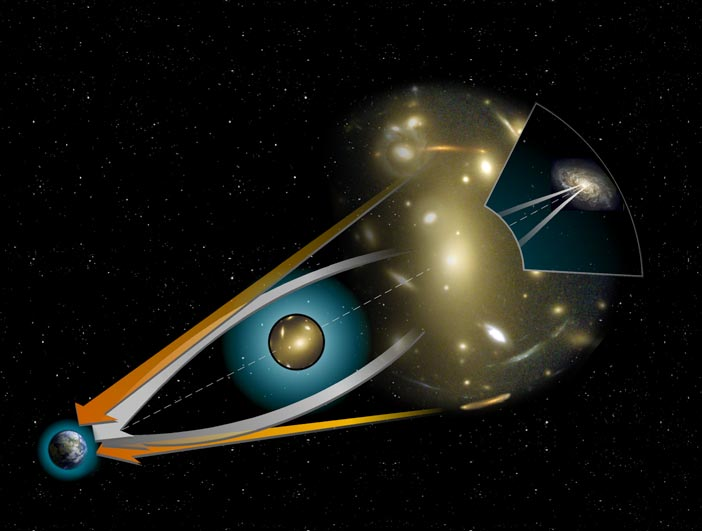
\includegraphics[scale=0.45]{Draw/lec10_6.png}
\end{center}
\caption{Gravitational lensing (Image credit: NASA)}
\label{fig:lec10_6}
\end{figure}

Notice that the deflection of light by the gravitational force of a massive body is a prediction of general relativity; Newton's law of gravitation predicts that the force bewteen a body and a photon is zero, since the photon is massless. Next we show how general relativity and a little bit of geometry allow us to calculate the mass a cluster that acts as a lens from the knowledge of other measurable quantities. We will consider the special case in which the source $S$, the lens $L$, and the observer $O$ are collinear, as shown in fig.\ \ref{fig:lec10_8}.
\begin{figure}[ht]
\begin{center}
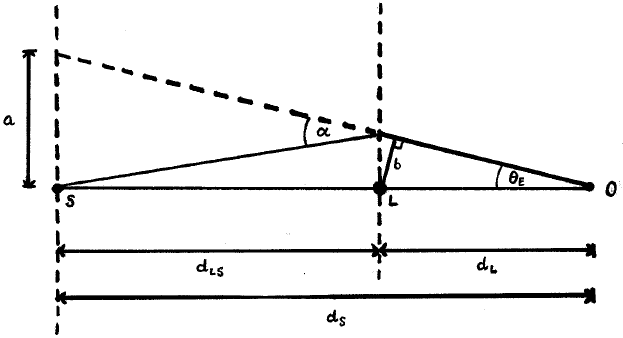
\includegraphics[scale=0.6]{Draw/lec10_8.png}
\end{center}
\caption{Gravitational lensing}
\label{fig:lec10_8}
\end{figure}

The trajectory of a light ray from $S$ to $O$ is (approximately) hyperbolic, but to simplify the diagram we have represented this trajectory by two straight lines (corresponding to the asymptotes of the hyperbola). General relativity predicts that the deflection angle, $\alpha$, is given by
\begin{equation} \label{eq:defl_angle1}
\alpha= \frac{4GM_L}{c^2 b},
\end{equation}
where $M_L$ is the mass of the lens, and $b$ is the {\it impact parameter}, which corresponds to the perpendicular distance between the lens and the asymptote that intersects the observer. Consider the right triangle with base $LO$; it is clear that we can relate $b$ to the angle $\theta_E$ by
\begin{equation}
b=d_L \sin\theta_E \simeq d_L \theta_E,
\end{equation}
where we have used the fact that $\theta_E$ is a small angle (which is true for all cosmological applications), so that the approximation $\sin\theta_E \simeq\theta_E$ holds.\footnote{If you have learned calculus, you will note that this approximation amounts to keeping the leading term in the Taylor expansion of the sine function.} Replacing $b$ in eq.\ (\ref{eq:defl_angle1}) we obtain
\begin{equation} \label{eq:defl_angle2}
\alpha= \frac{4GM_L}{c^2}\frac{1}{d_L \theta_E}.
\end{equation}
Next, consider the length $a$ in the diagram of fig.\ \ref{fig:lec10_8}. This is related to the angle $\theta_E$ by
\begin{equation} \label{eq:defl_angle3}
a=d_S \tan \theta_E \simeq d_S \theta_E,
\end{equation}
where we used the approximation $\tan\theta_E\simeq \theta_E$, valid for small $\theta_E$. On the other hand, $a$ is also related to the deflection angle $\alpha$ by
\begin{equation} \label{eq:defl_angle4}
a\simeq d_{LS} \tan\alpha \simeq d_{LS}\alpha.
\end{equation}
Combining eqs.\ (\ref{eq:defl_angle3}) and (\ref{eq:defl_angle4}) we obtain
\begin{equation}
d_S\theta_E = d_{LS}\alpha
\end{equation}
\begin{equation} \label{eq:defl_angle5}
\Rightarrow~~~~ \alpha = \frac{d_S\theta_E}{d_{LS}}.
\end{equation}
Finally, combining eqs.\ (\ref{eq:defl_angle2}) and (\ref{eq:defl_angle5}) we find
\begin{equation}
\frac{4GM_L}{c^2}\frac{1}{d_L \theta_E} = \frac{d_S\theta_E}{d_{LS}}
\end{equation}
\begin{equation} \label{eq:einstein_radius}
\Rightarrow~~~~\theta_E=\left( \frac{4GM_L}{c^2}\frac{d_{LS}}{d_L d_S} \right)^{1/2}.
\end{equation}
The angle $\theta_E$ is known as the {\it Einstein radius} (although, strictly speaking, it is an angle, not a radius). Eq.\ (\ref{eq:einstein_radius}) allows one to calculate the mass $M_L$ of the cluster that acts as a lens, from the knowledge of the quantities $\theta_E$, $d_L$, and $d_S$, which in many cases can be measured with good accuracy.

\subsection{Theories of dark matter}

\subsubsection{Modified Newtonian dynamics (MOND)}

All the evidence currently available that supports the existence of dark matter is based on the assumption that general relativity (or Newtonian gravity in the nonrelativistic cases) is the correct theory of gravity. Newton's law of gravitation has been experimentally tested with a high degree of precision, and the same is true for the relativistic corrections to this law predicted by general relativity. However, we do not have very precise experimental tests of gravity for objects at large distances which are subject to very weak gravitational forces. The theory of {\it modified Newtonian dynamics} (MOND) was introduced to explain the flat rotation curves observed for stars in spiral galaxies (see fig.\ \ref{fig:lec10_4}), without the need of an invisible dark matter. MOND postulates that the correct gravitational exerted by a mass $M$ on a particle of mass $m$, which are separated by a distance $R$, is given by
\begin{equation} \label{eq:mond1}
F_g=\frac{GM}{R^2}\frac{m}{\mu(a/a_0)},
\end{equation}
where $a$ is the acceleration of the particle,\footnote{Eq.\ (\ref{eq:mond1}) is, of course, a nonrelativistic law. Since MOND was first postulated a number of relativistic generalizations have been proposed.} and $a_0$ is known as Milgrom's acceleration constant, which is assumed to have a value of order $10^{-10}~\mathrm{m/s^2}$. The function $\mu(x)$ is assumed to have a shape similar to what is shown in fig.\ \ref{fig:lec10_9}. For $x\gg1$ it has the approximate value $\mu(x)\approx1$, while for $x\ll1$ one can approximate $\mu(x)\approx x$.
\begin{figure}[ht]
\begin{center}
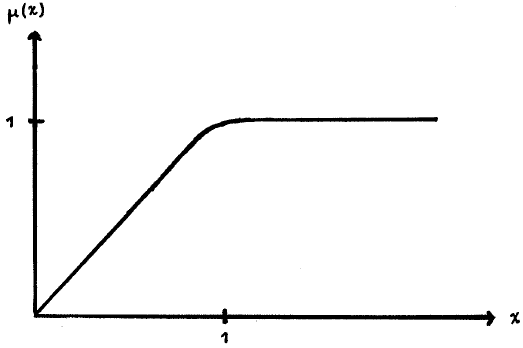
\includegraphics[scale=0.6]{Draw/lec10_9.png}
\end{center}
\caption{MOND}
\label{fig:lec10_9}
\end{figure}

Notice that the constance $a_0$ is very small, which means that on scales smaller than galactic scales we always have $a\gg a_0$, implying that $\mu(a/a_0)\approx 1$, and we recover Newton's law:
\begin{equation}
F_g\approx \frac{GMm}{R^2}.
\end{equation}
For example, consider the Earth moving around the Sun. The orbital speed of the Earth is approximately $v\approx 3\times10^4$ m/s, with a distance of $R\approx 10^8$ m from the Sun. This gives a centripetal acceleration of $a=v^2/R\sim 10~\mathrm{m/s^2}$, which of course is very much larger than $a_0$. The same is true for all objects on the scales of the solar system. Consider next the case of the Sun moving around the galactic center. The Sun moves with a speed of $v\approx 2\times10^5$ m/s at a distance of $R\approx 8$ kpc, giving a centripetal acceleration of $a\sim 2\times10^{-10}~\mathrm{m/s^2}$, which is now of the same order of magnitude as $a_0$.

For the stars on the outer edge of the galaxy we have that $a<a_0$, so according to MOND we have $\mu(a/a_0)\approx a/a_0$. Using this in eq.\ (\ref{eq:mond1}) gives the gravitational force:
\begin{equation}
F_g = \frac{GMm}{R^2}\frac{a_0}{a}.
\end{equation}
If we use that $a=v^2/R$ for a circular orbit, and equate $F_g$ to the centripetal force $F_c=mv2^/R$, we obtain
\begin{equation}
\begin{split}
\frac{GMm}{R^2}\frac{a_0 R}{v^2}&= m\frac{v^2}{R}\\
v&=\left(GMa_0\right)^{1/4}
\end{split}
\end{equation}
\begin{equation}
\Rightarrow~~~~ v\propto \mathrm{const.}
\end{equation}
We see that MOND indeed predicts that the rotational speeds of stars are independent of the radius $R$ at large distances from the galactic center, in agreement with observations. Although MOND has been successful in explaining the observations of dark matter in the context of galaxies, it has not been so successful in explaining the cosmological evidence, as well as the evidence of dark matter in galaxy clusters. Nevertheless, MOND and its relativistic generalizations remain an active field of research today, even though the experimental evidence seems to favor the theory of particle dark matter.

\subsubsection{Particle dark matter}

The most widely accepted explanation for the evidence of dark matter is that it is some kind of new particle. This theory of {\it particle dark matter} provides a framework in which all the observational evidence discussed above can be accurately explained. The problem with this theory, however, is that the dark matter particle has not been directly detected so far. We will see below that it cannot be one of the particles of the Standard Model, which means that a new theory of particle physics is needed in order to explain dark matter.

Before going into the particle physics aspects of dark matter, we can find an important constraint on the nature of the dark matter particle from cosmological observations. In the context of cosmology, we can classify the dark matter according to its average speed at the time of decoupling.\footnote{The concept of decoupling was discussed in chapters 6 and 7.} We can then distinguish two cases:
\begin{itemize}
\item Hot dark matter (HDM): it corresponds to particles that had a {\it relativistic} average speed ($v\sim c$) at the time of decoupling.
\item Cold dark matter (CDM): it corresponds to particle that had a {\it nonrelativistic} average speed ($v\ll c$) at the time of decoupling.
\end{itemize}
This classification is useful because it is directly related to the process of structure formation. Specifically, HDM gives rise to the so-called {\it top-down} scenario of structure formation, in which the largest structures in the universe form first, followed by structures of smaller scales. In this scenario, then, superclusters are the first structures to form. In contrast, CDM gives rise to the so-called {\it bottom-up} scenario of structure formation, in which the different structures grow hierarchically from the smallest to the largest ones. In this scenario galaxies form first, followed by clusters, and then superclusters, in a process driven by gravitational collapse. This is, in fact, what observations strongly suggest; at the present time we observe galaxies and clusters of galaxies in virial equilibrium, whereas superclusters are still undergoing gravitational collapse.

We are now ready to describe the properties that the dark matter particle must have in order to explain observations. The three main properties are the following:
\begin{itemize}
\item [(1)] It has to be electrically neutral (otherwise it would interact very efficient with light).
\item [(2)] It has to be stable (at least on cosmological timescales).
\item [(3)] It has to be cold (to explain the bottom-up process of structure formation).
\end{itemize}
It is not hard to see that there is no particle in the Standard Model that satisfies these three properties. Neutrons, for instance, satisfy (1) and (3), but not (2); neutrons have a lifetime of roughly 15 minutes (when they are not bound in atomic nuclei). Neutrinos, on the other hand, satisfy (1) and (2), but not (3); indeed, neutrinos would correspond to HDM, which is ruled out by observations as we have seen.

A simple calculation shows that neutrinos cannot be cold. If neutrinos were CDM, then their energy density today ($t=t_0$) would be
\begin{equation} \label{eq:neutrino_dm1}
\Omega_{DM}(t_0)= \frac{\rho_{\nu}(t_0)}{\rho_c(t_0)} \approx 0.22.
\end{equation}
Also, if neutrinos were nonrelativistic at the time of decoupling, they must also be nonrelativistic today. This means that their energy density is simply the product of the rest energy of a neutrino ($m_{\nu}c^2$) times the number of neutrinos per unit volume, denoted by $n_{\nu}$:
\begin{equation} \label{eq:neutrino_dm2}
\rho_{\nu}(t_0)=m_{\nu}n_{\nu}(t_0)c^2.
\end{equation}
Experimentally, we have that $n_{\nu}(t_0)\approx 4\times10^8~\mathrm{m^{-3}}$. Combining eqs.\ (\ref{eq:neutrino_dm1}) and (\ref{eq:neutrino_dm2}) we obtain a measurement of the rest energy of a neutrino:
\begin{equation}
m_{\nu}c^2\approx 4~\mathrm{eV}.
\end{equation}
However, neutrino experiments show that $m_{\nu}c^2 \lesssim 0.1$ eV, thus ruling out the neutrino as a dark matter candidate.

We conclude that there is no particle in the Standard Model that can serve as a dark matter candidate. As mentioned above, this implies that the dark matter particle must be part of a theory beyond the Standard Model. Several theories have been proposed in the past decades, although none of them has been experimentally verified so far. The dark matter candidates in these new theories are generically known as weakly interacting massive particles (or WIMPs).

\section{Dark energy}

\subsection{Observational evidence}

The main observational evidence for the existence of dark energy is that the expansion of the universe is accelerating. As we mentioned in the previous section, this evidence comes the observations of high-redshift type Ia supernovae (fig.\ \ref{fig:lec10_7}). Specifically, the observed relation between the apparent brightness and the redshift of distant supernovae cannot be explained unless one assumes the existence of dark energy.
\begin{figure}[ht]
\begin{center}
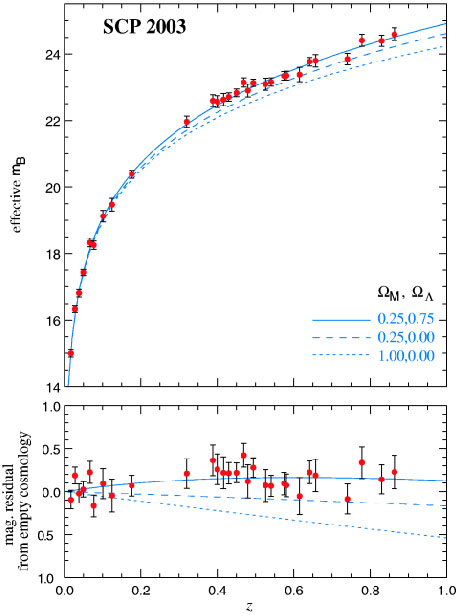
\includegraphics[scale=0.5]{Draw/lec10_7.png}
\end{center}
\caption{Observational evidence for dark energy (Image credit: Supernova Cosmology Project, 2003)}
\label{fig:lec10_7}
\end{figure}

In this course we have been assuming that the dark energy density is independent of the scale factor, implying that it remains constant in time. This assumption is well-motivated, as it follows from the existence of a cosmological constant (see below). However, we would like to show that the dark energy density does not need to be constant in order to produce an accelerated expansion. Consider a form of energy that decreases with the scale factor $a(t)$ in the following way:
\begin{equation} \label{eq:w0}
\rho_w(t)=\frac{\rho_w(t_0)}{a(t)^{3(1+w)}},
\end{equation}
where $w$ is some constant, and we used that $a(t_0)=1$ by definition (with $t_0$ the present time). Different choices of the parameter $w$ corresponds to different forms of energy. For instance, $w=0$ implies that $\rho_w\propto 1/a^3$, and corresponds to matter; $w=1/3$ implies that $\rho_w\propto 1/a^4$, and corresponds to radiation.

Suppose that at late times this form of energy $\rho_w(t)$ dominates the universe, so that the Friedmann equation can be written as
\begin{equation} \label{eq:w1}
\left(\frac{\dot{a}}{a}\right)^2= \frac{8\pi G}{3c^2}\frac{\rho_w(t_0)}{a^{3(1+w)}}.
\end{equation}
Solving for $\dot{a}$ we obtain
\begin{equation} \label{eq:w2}
\dot{a}=\left(\frac{8\pi G}{3c^2}\rho_w(t_0)\right)^{1/2} \frac{1}{a^{(1+3w)/2}}.
\end{equation}
Taking the time derivative of this last equation we get
\begin{equation} \label{eq:w3}
\ddot{a}=-\frac{(1+3w)}{2}\left(\frac{8\pi G}{3c^2}\rho_w(t_0)\right)^{1/2} \frac{\dot{a}}{a^{3(1+w)/2}}
\end{equation}
\begin{equation} \label{eq:w4}
\Rightarrow~~~~ \ddot{a}=-\frac{(1+3w)}{2}\left(\frac{8\pi G}{3c^2}\rho_w(t_0)\right) \frac{1}{a^{2+3w}}
\end{equation}

\par\vspace{\baselineskip}

{\bf Exercise.} Complete the intermediate steps in the derivation of eq.\ (\ref{eq:w4}), starting from eq.\ (\ref{eq:w1}).

\par\vspace{\baselineskip}

This last result is useful because it provides a way to determine whether the expansion rate due to the energy density $\rho_w$ is accelerated or not. Recall that the expansion of the universe is accelerated if $\ddot{a}>0$. Eq.\ (\ref{eq:w4}) tells us that this will be true provided that $(1+3w)<0$, or $w<-1/3$. On the other hand, we see from eq.\ (\ref{eq:w0}) that we must require that $(1+w)\geq0$, or $w\geq-1$, for otherwise $\rho_w$ would {\it increase} as the universe expands.\footnote{The possibility of having $w<-1$ corresponds to the so-called {\it phantom energy}, which is sometimes studied in theories of the very early universe as alternatives to inflation.} We conclude that the parameter $w$ that corresponds to the dark energy must satisfy the following:
\begin{equation} \label{eq:wbounds}
-1\leq w <-1/3.
\end{equation}

\subsection{Theories of dark energy}

The theories of dark energy can be divided into three classes. The first and simplest one is that the dark energy is due to a cosmological constant. Secondly, there is the possibility that the dark energy corresponds to a dynamical field, which at late times evolves with a nearly constant energy density. A third possibility assumes that general relativity is modified on cosmological scales in such a way that the universe accelerates at late times without the need of a new form of energy. After briefly reviewing the relation between the cosmological constant and dark energy, we will describe two examples of theories that belong to the second and third alternative explanations that we mentioned.

\subsubsection{Cosmological constant}

The cosmological constant, denoted by $\Lambda$, was originally introduced by Einstein in order to obtain a solution to his field equations corresponding to a static universe. Specifically, the contribution to the energy density that comes from the constant $\Lambda$ is
\begin{equation}
\rho_{\Lambda}=\frac{\Lambda c^2}{8\pi G}.
\end{equation}
We see that $\rho_{\Lambda}$ is constant in time and independent of the scale factor, so the cosmological constant indeed corresponds to dark energy with parameter $w=-1$; see eqs.\ (\ref{eq:w0}) and (\ref{eq:wbounds}).

Einstein later abandoned this idea of introducing $\Lambda$, after becoming aware of the observations made by Hubble that the universe is in fact expanding. However, after the development of quantum field theory it was realized that fields possess a {\it vacuum energy}, whose energy density does not depend on the expansion of the universe, and should therefore act as a cosmological constant. This fact, in addition to the recent observations of the accelerated expansion, has convinced many physicists that the dark energy is due to a cosmological constant. This picture currently faces an important problem, known as the {\it cosmological constant problem}, related to the fact that theory and experiment disagree enormously about the value of $\rho_{\Lambda}$. On the one hand, observations suggest that, in order to explain the present expansion rate, the dark energy density should be
\begin{equation}
\rho_{\Lambda}=\rho_c(t_0)\Omega_{\Lambda}(t_0)\sim 10^9~\mathrm{eV/m^3}.
\end{equation}
On the other hand, quantum mechanics (as we currently understand it) predicts a vacuum energy density that is much larger:
\begin{equation}
\rho_{\mathrm{vacuum}}\sim 10^{133}~\mathrm{eV/m^3}.
\end{equation}
This implies that $\rho_{\mathrm{vacuum}}\sim 10^{124}\rho_{\Lambda}$, a difference of 124 orders of magnitude! This is often regarded as the biggest disagreement between theory and experiment in the history of physics.

\subsubsection{Quintessence}

Quintessence is a hypothetical scalar field (denoted by $q$) that would mediate a fifth fundamental force. During the radiation-dominated epoch quintessence behaves like a relativistic fluid with a parameter $w_q=1/3$ (see eq.\ (\ref{eq:w0})), but it is nevertheless subdominant when compared to the usual radiation (photons and neutrinos), so that the predictions of the standard cosmological model are not affected by it. After the universe becomes matter-dominated quintessence changes its behavior, and begins to evolve with a corresponding parameter $w_q\simeq -1$, so that it effectively behaves as dark energy. It has been shown that in some specific models quintessence can have a present energy density that is in agreement with observations.

\subsubsection{DGP model}

A different possibility to explain the observed cosmic acceleration was proposed by Dvali, Gabadadze, and Porrati, and is known as the DGP model. It states that our universe is 3-dimensional hypersurface (called the {\it brane}) embedded in a 4-dimensional space (called the {\it bulk}); see fig.\ \ref{fig:lec10_10}. In this model gravity is really a 4-dimensional force (unlike the Standard Model forces, which are confined to the 3-dimensional brane), which nevertheless behaves as 3-dimensional on scales shorter than cosmological, thus effectively reproducing general relativity. However, on cosmological scales and beyond, general relativity is modified by the fact that the geometry of the brane becomes important, and in fact, it has been shown that the bending of the brane can have the effect of an accelerated expansion as seen from the point of view of our 3-dimensional universe.
\begin{figure}[ht]
\begin{center}
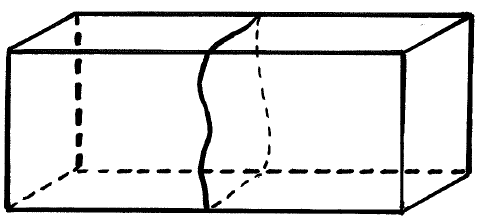
\includegraphics[scale=0.55]{Draw/lec10_10.png}
\end{center}
\caption{DGP model}
\label{fig:lec10_10}
\end{figure}